%%____________________________________________________________________________||

\section{Background estimation for processes with genuine \met}
\label{sec:backgroundmet}

Once all the signal region selection requirements have been imposed,
the contribution from QCD multijet events is expected to be
negligible, as demonstrated in Sec.~\ref{sec:background_qcd}. 
In the absence of multijet events, the background counts in the signal region arise from
SM processes with significant \met in the final state. In events with
low statistics of jets and b-quark jets, the largest backgrounds with
genuine \met are from the associated production of W or Z bosons with
jets, followed by either the weak decays \znunu or \wtaunu, where the
$\tau$ decays hadronically and is identified as a jet; or by leptonic
decays that are not rejected by the dedicated electron or muon
vetoes. The veto of events containing isolated tracks is efficient at
further suppressing these backgrounds as well as the single-prong
hadronic decay of the tau lepton. At higher jet and b-quark jet
multiplicities, top quark production followed by semileptonic weak top
quark decay becomes important.  Residual contributions from processes
such as single-top-quark, $\ttbar$V or $\ttbar$H, diboson, and
Drell-Yan production are also expected. These SM processes are
collectively referred to as the non-multijet backgrounds.

\subsection{Additional corrections to simulated samples}
\label{sec:mc-corrections}

The simulated samples are normalised using the most accurate cross
section calculations currently available, usually with
next-to-leading-order (NLO) accuracy~\ref{sec:datasets}. 
To model the effect of pileup, the simulated events are generated with a nominal distribution
of pp interactions per bunch crossing, which are then reweighted
to match the pileup distribution as measured in data, as described in~\ref{sec:pileup-reweighting}

Additional re-weighting procedures applied to the simulated samples are described in the following.

\subsubsection{Normalisation corrections from a \mht sideband}
\label{sec:sideband-corrections}

In the high-\scalht, high-\etmiss corner of the phase space used in this search, the normalisations of the MC samples do not necessarily agree with the observation. 
Moreover, the cross section is known only to a limited number of perturbative orders and additional corrections could be in principle sizeable. \\
The analysis strategy for the background predictions is built in such a way to be mildly, if not negligibly, dependent on these corrections. 
The backgrounds are estimated from control regions in data, and the effect of cross section corrections on the transfer factors is expected to largely cancel out, 
because the background composition is very similar between the signal region and the control regions used to estimate each background. \\
However, the ``data-driven'' tests described in Sec.~\ref{sec:closure-tests} would benefit from a better control of the normalisation of MC samples, 
since more aggressive extrapolations are carried on there with respect to the background predictions in the analysis. 

In this section a procedure is described to derive process-dependent ``sideband corrections'' 
by means of a likelihood fit using the data in the control regions. 
The sideband corrections are derived after all the other corrections to the MC and data are applied, 
such as trigger efficiency, data/MC scale factors (b-tag, lepton ID/isolation, etc.) and jet energy scale. 
The sideband corrections are applied and propagated to all the steps of the analysis.\\
No uncertainty is considered for these corrections as any inaccuracy is already accounted 
for in the data-driven tests described in Sec.~\ref{sec:closure-tests} and would result in inflated systematics. 

To take advantage of the full phase space of the sidebands a simultaneous 
fit is used to derive the corrections for \wj, \zj, \ttbar, using the $100<\mht<130$ GeV sideband. 
The sideband is binned identically to the control region in \njet, \nb and \scalht and a floating 
parameter per relevant process encodes the correction for that process (fully correlated across all bins).
The \wj and \ttbar processes are mainly constrained by the \mj sideband while the \zj process is 
constrained by the \mmj sideband. The values of the corrections and uncertainties
given by the fit are shown in Table~\ref{tab:sbCorrsFromFit}.\\
The correction derived for \zj is also applied to the \znunu sample. 

\begin{table}[!h]
  \scriptsize
  \centering
  \topcaption{Cross section corrections for SM backgrounds derived with fit to sidebands in data.}
  \label{tab:sbCorrsFromFit}
  \begin{tabular}
    {cllc}
    \hline\hline
    \textbf{Process} & \textbf{Sideband} & \textbf{Selection} & \textbf{Corrrection} \\
    \hline
    \wj & $100 < \mht < 130 \, \mathrm{GeV}$ & \mj& $1.13 \pm 0.01$ \\
    \zj & $100 < \mht < 130 \, \mathrm{GeV}$ & \mmj& $1.08 \pm 0.01$ \\
    \ttbar + jets & $100 < \mht < 130 \, \mathrm{GeV}$ & \mj, \mmj  & $0.91 \pm 0.01$ \\
    \hline \hline
  \end{tabular}
\end{table}

\subsubsection{Estimate of non-prompt contribution in \gj events}
\label{sec:photon-purity}

The contribution from non-prompt photons in the \gj control region~\ref{sec:photoncontrolSelection} 
is expected to be small after the tight ID selection~\ref{sec:photon-id}, the photon acceptance requirements 
and the \alphat and $\Delta R (\gamma,\mathrm{jet})$ cuts. 
Nevertheless a data-driven estimation of the non-prompt photons has been developed. 
%in order to assess the agreement with the simulation and eventually correct the latter 
%to better match the data. 
The non-prompt contribution is provided by the QCD MC samples. The
expected counts from MC are normalised (i.e. corrected) to data in a
sideband enriched in non-prompt photons (i.e. ``fakes''). These
corrections are determined as a function of photon \Pt to provide a
data-driven photon-\Pt-dependent estimate of the non-prompt
contribution to the \gj sample. No $\eta$ dependence is considered, as
the analysis only considers barrel photons ($|\eta| < 1.45$) and no
strong dependence is expected. 

A double-sideband is considered by relaxing the photon ID and isolation, 
specifically the $\sigma_{i\eta i\eta}$ requirement and the charged hadron isolation requirement. 
The details of the definition of the sideband are listed in Tab.~\ref{tab:phoPurity-sideband}. 
The $\sigma_{i\eta i\eta}$ distribution in the charged hadron isolation sideband is shown for two 
photon \pt bins in Fig.~\ref{fig:chHadIsoSideband}.

\begin{table}[h!]
  \topcaption{Summary of the photon selection for the sideband used to estimate the non-prompt component. }
  \label{tab:phoPurity-sideband}
  \centering
  \footnotesize
  \begin{tabular}{ ccccc }
    \hline
    \hline
    Variable & Nominal selection & Sideband selection & Sideband up variation & Sideband down variation \\
    \hline
    $\sigma_{i\eta i\eta}$   & $<0.010$ & $>0.011$ & $>0.012$ & $>0.010$ \\
    charged hadron isolation & $<0.76$  & $>1.00$  & $>1.50$  & $>0.76$  \\ 
    \hline
    \hline
  \end{tabular}
\end{table}

\begin{figure}[h!]
  \centering
  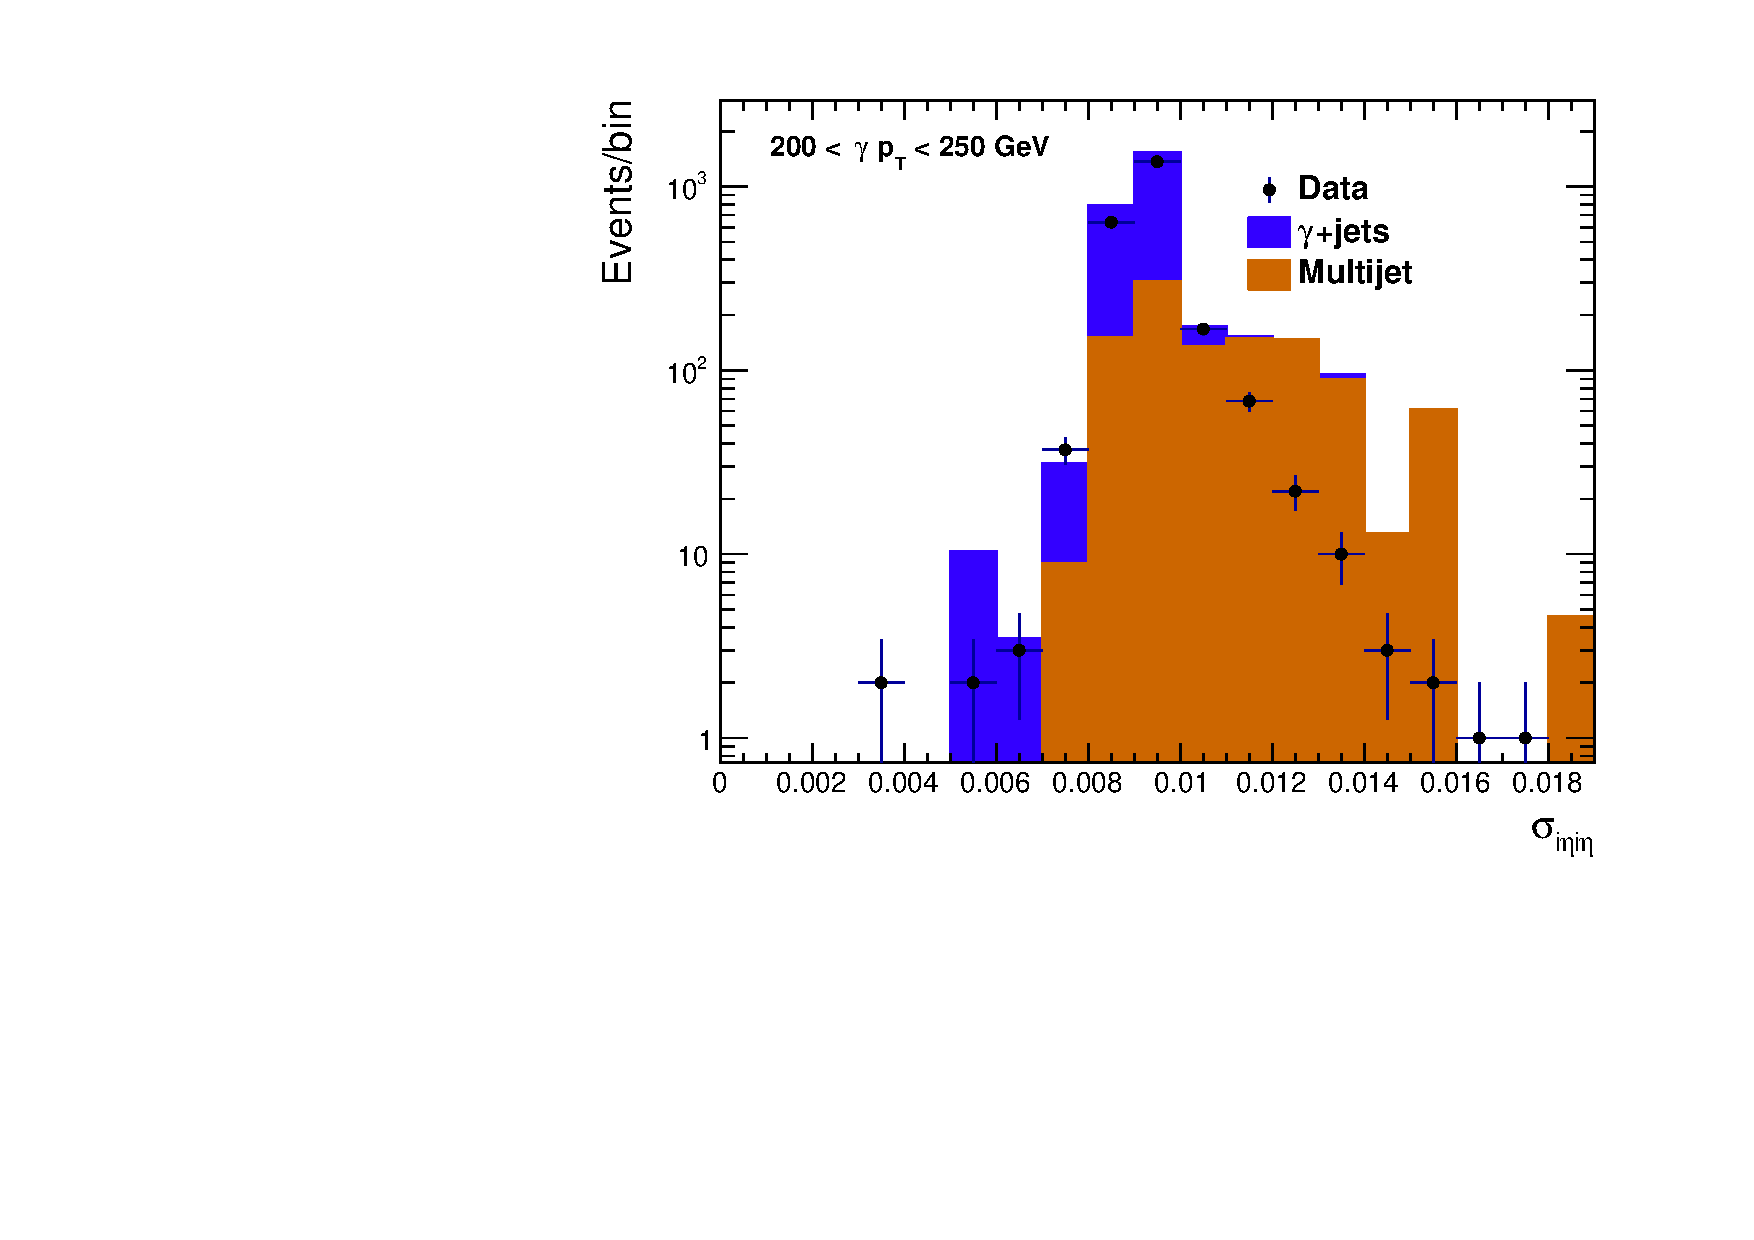
\includegraphics[width=0.45\textwidth]{figures/photonpurity/sigmaIetaIeta_chHadIsoSB_all_gammaPt_200_250_nominal} 
  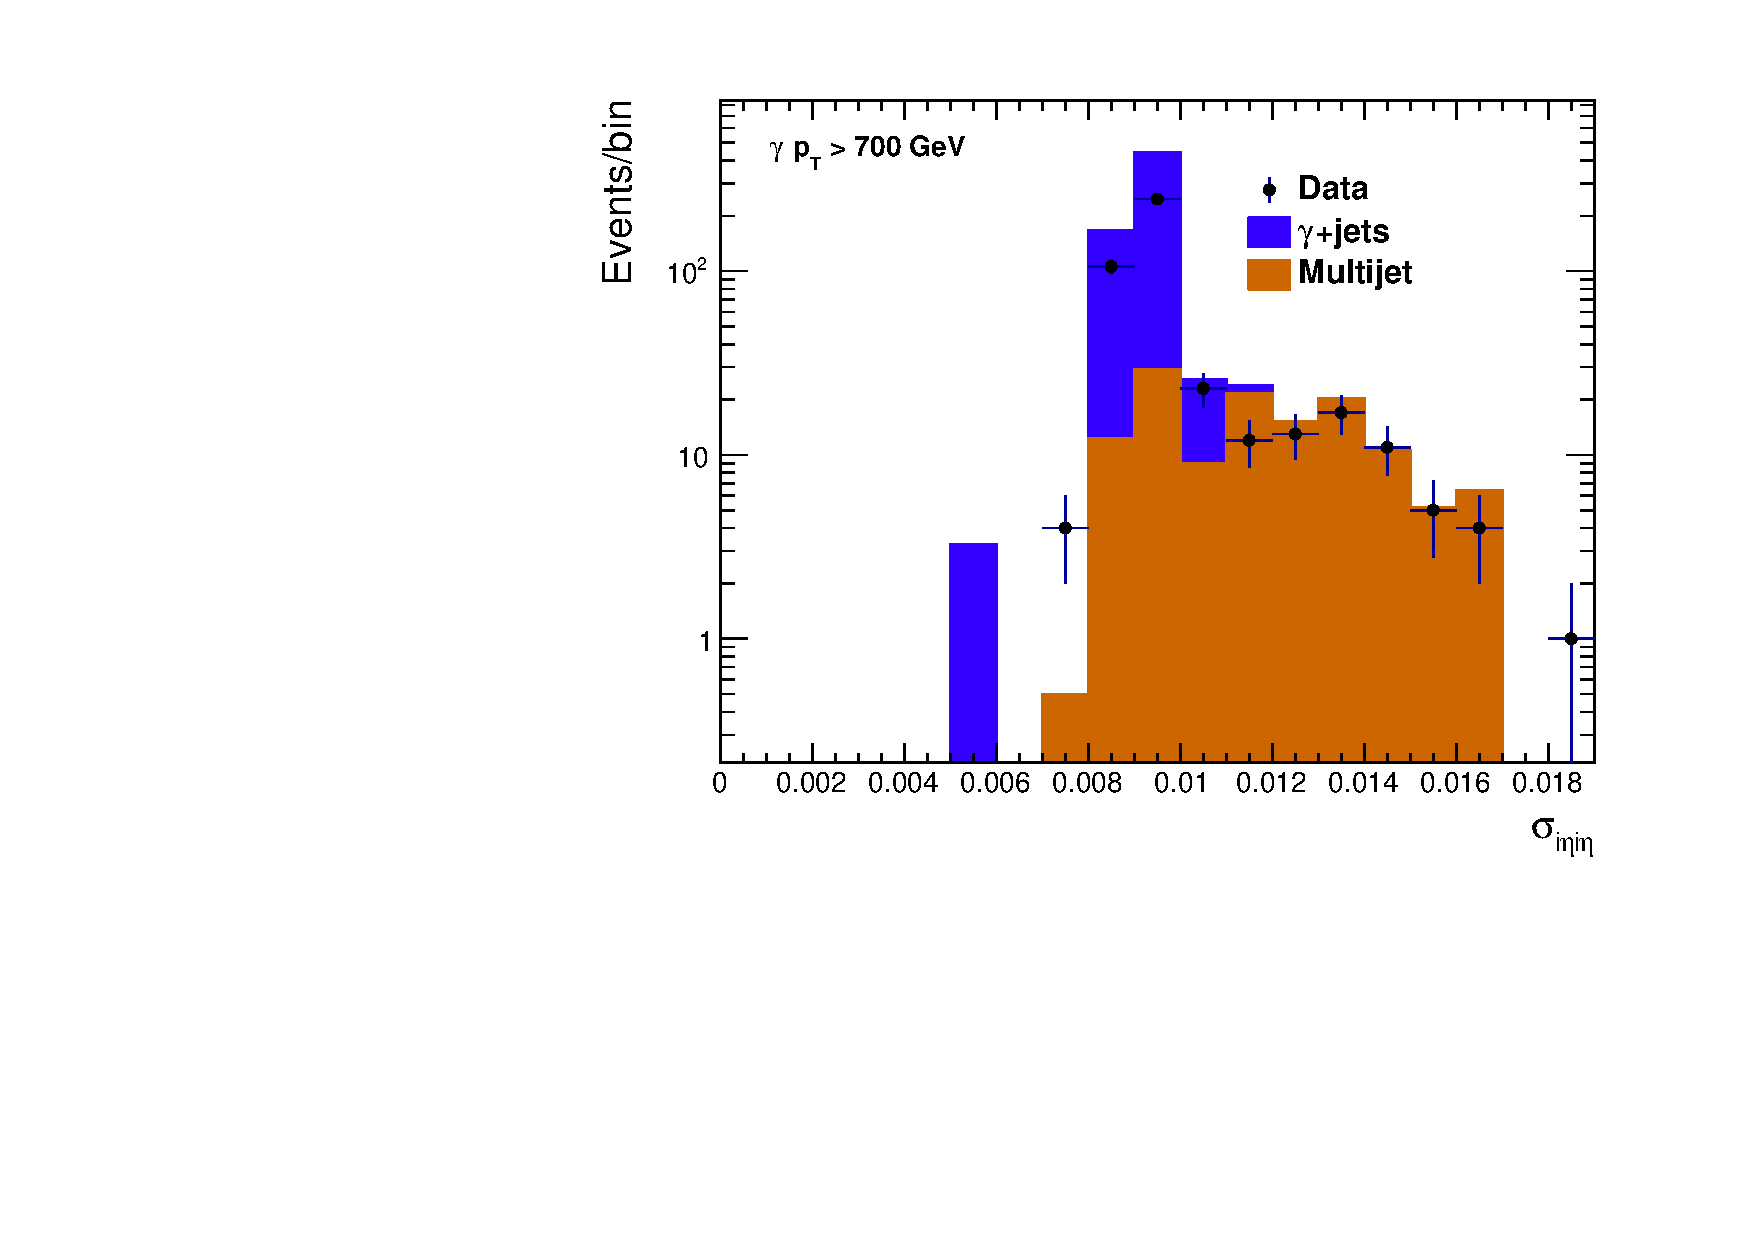
\includegraphics[width=0.45\textwidth]{figures/photonpurity/sigmaIetaIeta_chHadIsoSB_all_gammaPt_700_999999_nominal} 
  \caption{\label{fig:chHadIsoSideband} 
  The $\sigma_{i\eta i\eta}$ distribution in the charged hadron isolation sideband for two photon \pt bins. }
\end{figure}

The data in the sideband are used to normalise the non-prompt component in simulation, 
after subtracting the small contribution ($<5$\%) from prompt photons taken from simulation. 
All the statistical uncertainties, from both data and MC counts are propagated. \\
In order to assess the systematic uncertainties in the modelling of $\sigma_{i\eta i\eta}$ 
and charged hadron fraction the boundaries of the sideband are shifted from the 
nominal definition in both directions and for both variables, for a total of 4 different variations. 
The details on the sideband definitions for the systematic variations are given in Tab.~\ref{tab:phoPurity-sideband}. 
The 4 variations are conservatively summed in quadrature to obtain the total uncertainties. 
The systematic uncertainties ranges between 10-80\% depending on the photon \pt, 
and is larger at low photon \pt.

The relative contribution of non-prompt photons in the \gj control region 
is shown as a function of the photon transverse momentum in Fig.~\ref{fig:photon-purities}.
The study confirms a very high photon purity for the selection applied in this analysis, 
with a ``fake'' photon component between 1-3\%. 

\begin{figure}[h!]
  \centering
  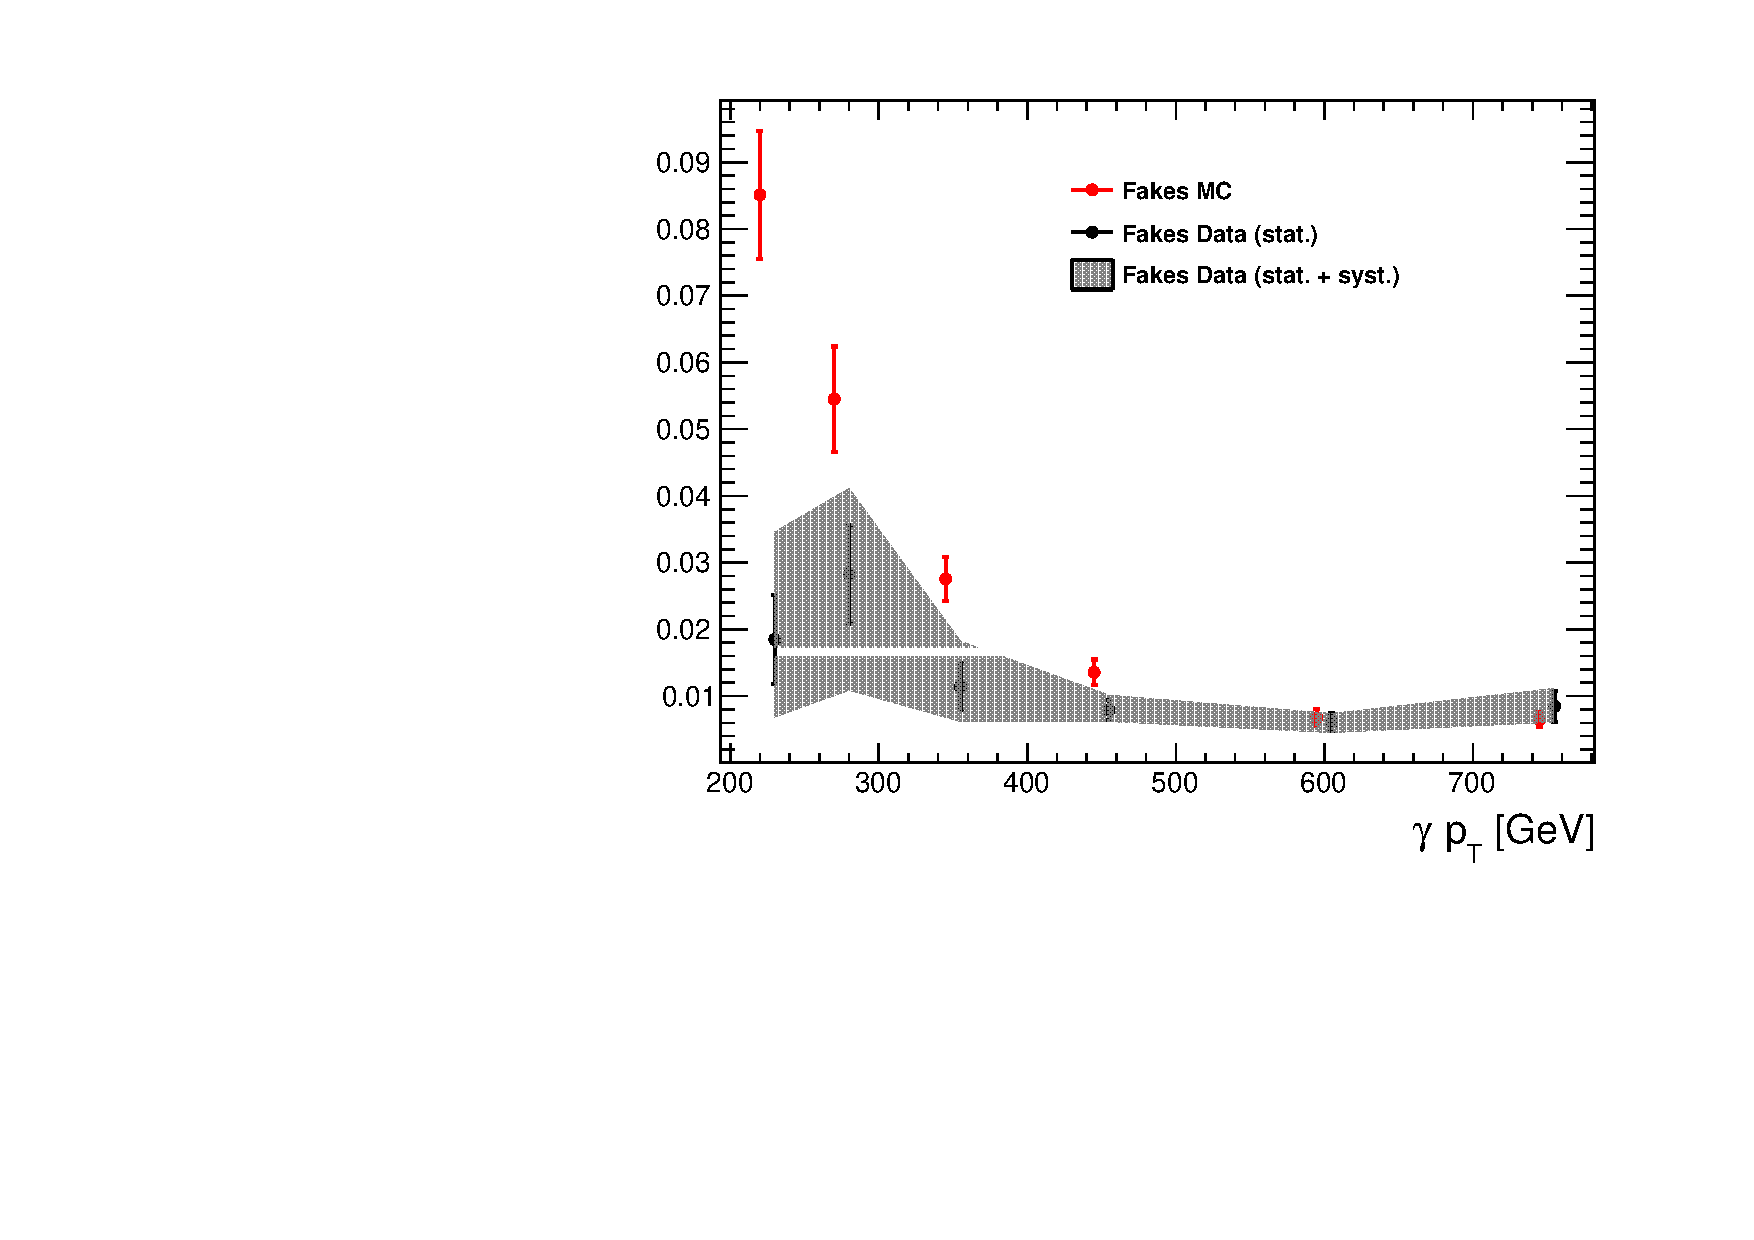
\includegraphics[width=0.45\textwidth]{figures/photonpurity/fakes} 
  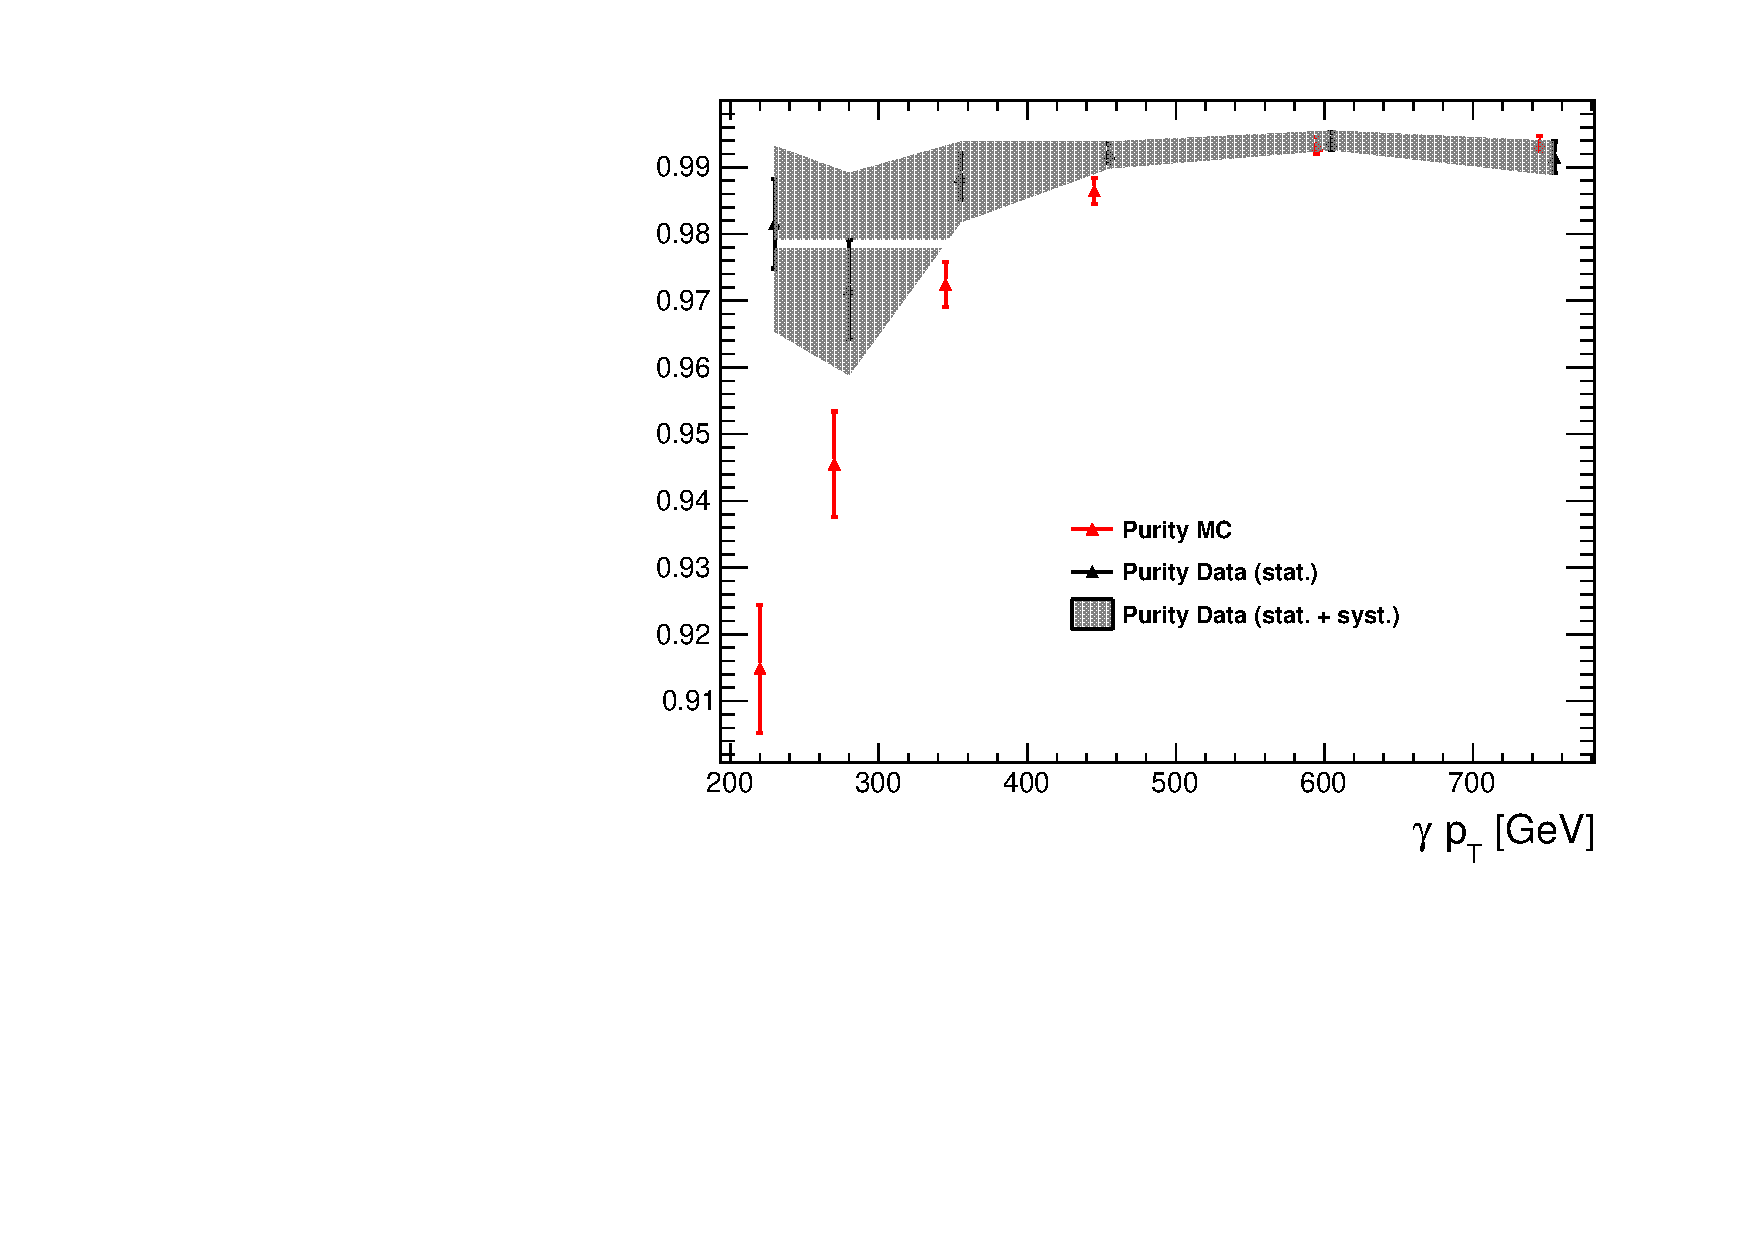
\includegraphics[width=0.45\textwidth]{figures/photonpurity/purity} 
  \caption{\label{fig:photon-purities} 
  The relative contribution of non-prompt photon (left) and
  the photon purity (right) as a function of the photon \pt, 
  comparing simulation with the data-driven estimation. }
\end{figure}

Given the significant discrepancy observed between the prediction from simulation and data, 
especially at low photon \pt, 
the non-prompt component in simulation is re-weighted as a function of the photon transverse momentum 
and both the statistical and systematic uncertainties are propagated to these correction factors. 


\subsubsection{Correction to \texorpdfstring{\gj}{photon+jets} cross section}
\label{sec:gj-kfactor}

The \gj cross section used in this analysis is calculated at leading
order, unlike other processes like \ttj (next-to-next-to leading
order) or \zj and \wj (next-to leading order).  A data-driven
procedure is developed to derive a ``k-factor'' for the \gj cross
section by comparing the yields in the \gj and \mmj control regions.
An inclusive correction of 1.39 is derived from the ratio of the event
yields in the two
control regions and is applied to the \gj MC sample. \\
In order to assess the uncertainty on this correction, the systematic
sources affecting the acceptance in the \mmj control region are varied
and the effect on the event yields is derived.  They include lepton
trigger, ID, isolation, tracking efficiency and jet energy
corrections.  The total systematic uncertainty, obtained by summing in
quadrature each independent variation, is 4\% and it's propagated to
the likelihood fit.  Residual discrepancy in the $Z/\gamma$ ratio as a
function of \scalht and \njet are assessed through the data-driven
test described in Sec.~\ref{sec:closure-tests}.


%% \subsection{The ``transfer factor'' method}
%% \label{sec:ewk-method}

%% The method used to estimate the aforementioned SM background
%% contributions in the hadronic signal region relies on the use of a
%% transfer factor (TF) determined from MC samples to transform the
%% observed yield in a given \scalht, jet (\njet) and b-tag (\nb)
%% multiplicity bin of a control sample, $\nobs^{\rm
%%   control}(\njet,\nb,\scalht)$, into a predicted yield for the
%% corresponding bin of the hadronic signal region, $\npre^{\rm
%%   signal}(\njet,\nb,\scalht)$. The choice of \njet and \nb~event
%% categorisation and \scalht binning in the control samples is identical
%% to that for the signal region, as defined in
%% Sec.~\ref{sec:selection}. 

%% Each transfer factor is simply a ratio of the yields obtained from MC
%% simulation for the same bin of the signal region and a given control
%% sample:

%% \begin{equation}
%%   \label{equ:tf-ratio}
%%   {\rm TF} = \frac{N_{\rm MC}^{\rm signal}(\njet,\nb,\scalht)}{N_{\rm
%%       MC}^{\rm control}(\njet,\nb,\scalht)} 
%% \end{equation}

%% In this way, predictions of background counts from SM processes can be
%% made based on the various control samples:

%% \begin{equation}
%%   \label{equ:pred-method}
%%   \npre^{\rm signal}(\njet,\nb,\scalht) = \frac{N_{\rm MC}^{\rm
%%       signal}(\njet,\nb,\scalht)}{N_{\rm MC}^{\rm
%%       control}(\njet,\nb,\scalht)} \times \nobs^{\rm
%%     control}(\njet,\nb,\scalht)   
%% \end{equation}

%% When constructing the transfer factors, the MC expectations for the
%% following SM processes are considered: W + jets ($N_{\rm W}$), \ttbar
%% + jets ($N_{\ttbar}$), \znunu\ + jets ($N_{\znunu}$), DY + jets
%% ($N_{\mathrm DY}$), \gj ($N_\gamma$), single top + jets
%% production via the $s$, $t$, and $tW$-channels ($N_{\rm top}$), $WW+$~jets, $WZ~+$~jets, and $ZZ + \textrm{jets}$ ($N_{\rm di-boson}$), and $\ttbar$V or
%% $\ttbar$H ($N_{\rm {\ttbar}X}$). Details on the MC
%% samples used are given in Sec.~\ref{sec:datasets}. All MC samples
%% are normalised to the integrated luminosity of the appropriate data
%% sample.

%% The selection criteria for the data control samples closely resemble
%% those for the signal region, differing mainly through the use of a
%% lepton or photon object {\it tag} (that is ignored in the calculation
%% of jet-based kinematic variables such as \scalht, \mht, \alphat, \etc)
%% and minimal additional kinematic requirements (\eg invariant or
%% transverse mass windows) to obtain W, Z, and \ttbar-enriched event
%% samples. The same selection criteria are designed to suppress signal
%% contamination in the control samples so that unbiased data-driven
%% estimates for the SM backgrounds in the signal region can be
%% made. More detail on the selection criteria can be found in Sec.~\ref{sec:selection}.

%% The transfer factors account for differences in cross sections and
%% branching ratios, acceptance and reconstruction efficiencies, and/or
%% kinematic requirements between the signal and control regions. Any
%% dependence on \njet, \nb, or \HT is largely attributable to
%% differences in acceptance due to the presence or otherwise of \alphat
%% or \mht requirements.

%% Many systematic effects are expected to cancel largely in the transfer
%% factor. However, a systematic uncertainty is assigned to each transfer
%% factor to account for theoretical uncertainties and effects such as
%% the mismodelling of kinematics (\eg acceptances) and instrumental
%% effects (\eg reconstruction efficiencies).

%% In the end, a fitting procedure that provides the final result is
%% defined formally by the likelihood model described in
%% Sec.~\ref{sec:likelihood}. In summary, the observation in each bin
%% (defined in terms of the variables \njet, \nb, and \scalht) of the
%% signal sample is modelled as Poisson-distributed about the sum of a SM
%% expectation (and a potential signal contribution). The components of
%% this SM expectation are related to the expected yields in the control
%% samples via transfer factors derived from simulation. The observations
%% in each bin (again defined by \njet, \nb, and \scalht) of the control
%% samples are similarly modelled as Poisson-distributed about the
%% expected yields for each control sample. In this way, for a given
%% bin, the observed yields in the signal and control samples are
%% connected via the transfer factors derived from simulation. 

%% The transfer factors are shown in Tables~\ref{tab:tf_mu_zinv_sym}-
%% \ref{tab:tf_mumu_zinv_mono}. The procedure to determine the systematic
%% uncertainties associated with these transfer factors is described in
%% Sec.~\ref{sec:systematics}.


%% The transfer factors are shown in tables below.

%% \begin{table}[h!]
\tiny
\centering
\caption{Transfer factors from the \mj control region to the \zInv~ background for symmetric categories.\label{tab:tf_mu_zinv_sym}}
\scalebox{0.85}{\begin{tabular}{ccccccccc}
	\hline\hline
	& \multicolumn{8}{c}{\scalht (\gev)} \\ 
	 (\njet,  \nb) & 200-250 & 250-300 & 300-350 & 350-400 & 400-500 & 500-600 & 600-800 & 800-$\infty$ \\ [0.8ex] 
\hline
	(2, 0) & $1.00\pm 0.02$ & $0.76\pm 0.01$ & $0.57\pm 0.01$ & $0.39\pm 0.01$ & $0.30\pm 0.01$ & $0.21\pm 0.01$ & $0.14\pm 0.00$ & $0.28\pm 0.01$ \\[0.5ex] 
	(2, 1) & $0.48\pm 0.03$ & $0.51\pm 0.02$ & $0.54\pm 0.03$ & $0.44\pm 0.03$ & $0.33\pm 0.02$ & $0.26\pm 0.02$ & $0.20\pm 0.01$ & $0.43\pm 0.03$ \\[0.5ex] 
	(2, 2) & $0.68\pm 0.13$ & $0.77\pm 0.14$ & $0.68\pm 0.14$ & $0.48\pm 0.12$ & $0.33\pm 0.07$ & $0.37\pm 0.12$ & $0.22\pm 0.06$ & -- \\[0.5ex] 
	(3, 0) & $0.19\pm 0.08$ & $0.45\pm 0.01$ & $0.53\pm 0.01$ & $0.53\pm 0.01$ & $0.42\pm 0.01$ & $0.27\pm 0.01$ & $0.19\pm 0.00$ & $0.26\pm 0.00$ \\[0.5ex] 
	(3, 1) & -- & $0.10\pm 0.01$ & $0.16\pm 0.01$ & $0.17\pm 0.01$ & $0.20\pm 0.01$ & $0.18\pm 0.01$ & $0.15\pm 0.01$ & $0.26\pm 0.01$ \\[0.5ex] 
	(3, 2) & -- & $0.08\pm 0.02$ & $0.10\pm 0.01$ & $0.08\pm 0.01$ & $0.08\pm 0.01$ & $0.07\pm 0.01$ & $0.07\pm 0.01$ & $0.14\pm 0.02$ \\[0.5ex] 
	(3, $\ge3$) & -- & -- & -- & -- & $0.03\pm 0.03$ & -- & -- & -- \\[0.5ex] 
	(4, 0) & -- & -- & $0.51\pm 0.03$ & $0.54\pm 0.02$ & $0.44\pm 0.01$ & $0.33\pm 0.01$ & $0.23\pm 0.00$ & $0.24\pm 0.00$ \\[0.5ex] 
	(4, 1) & -- & -- & $0.13\pm 0.01$ & $0.11\pm 0.01$ & $0.11\pm 0.00$ & $0.11\pm 0.01$ & $0.10\pm 0.00$ & $0.17\pm 0.01$ \\[0.5ex] 
	(4, 2) & -- & -- & $0.07\pm 0.02$ & $0.04\pm 0.01$ & $0.05\pm 0.00$ & $0.04\pm 0.00$ & $0.05\pm 0.00$ & $0.09\pm 0.01$ \\[0.5ex] 
	(4, $\ge3$) & -- & -- & -- & $0.06\pm 0.04$ & $0.07\pm 0.02$ & $0.03\pm 0.02$ & $0.03\pm 0.01$ & $0.12\pm 0.05$ \\[0.5ex] 
	($\ge5$, 0) & -- & -- & -- & $0.31\pm 0.04$ & $0.36\pm 0.01$ & $0.27\pm 0.01$ & $0.19\pm 0.00$ & $0.18\pm 0.00$ \\[0.5ex] 
	($\ge5$, 1) & -- & -- & -- & $0.07\pm 0.02$ & $0.07\pm 0.01$ & $0.05\pm 0.00$ & $0.05\pm 0.00$ & $0.06\pm 0.00$ \\[0.5ex] 
	($\ge5$, 2) & -- & -- & -- & $0.01\pm 0.01$ & $0.03\pm 0.00$ & $0.02\pm 0.00$ & $0.02\pm 0.00$ & $0.03\pm 0.00$ \\[0.5ex] 
	($\ge5$, $\ge3$) & -- & -- & -- & -- & $0.03\pm 0.02$ & $0.02\pm 0.01$ & $0.03\pm 0.01$ & $0.03\pm 0.01$ \\[0.5ex] 
	\hline
	\hline
\end{tabular}}
\end{table}

%% \begin{table}[h!]
\tiny
\centering
\caption{Transfer factors from the \mj control region to the \zInv~ background for asymmetric categories. The letter ``a'' in jet \eg ``2a''  indicates the asymmetric jet bins. All entries are non-zero but are truncated to one decimal place.\label{tab:tf_mu_zinv_asym}}
\begin{tabular}
{ccccccccc}
	\hline\hline
&	& \multicolumn{8}{c}{\scalht (\gev)} \\ 
	 (\njet,  \nb) & 200-250 & 250-300 & 300-350 & 350-400 & 400-500 & 500-600 & 600-800 & 800-$\infty$ \\ [0.8ex] 
\hline
	(2a, 0) & $0.55^{+ 0.01 }_{- 0.01 }$ & $0.34^{+ 0.01 }_{- 0.01 }$ & $0.30^{+ 0.01 }_{- 0.01 }$ & $0.30^{+ 0.01 }_{- 0.01 }$ & $0.30^{+ 0.01 }_{- 0.01 }$ & $0.28^{+ 0.01 }_{- 0.01 }$ & $0.25^{+ 0.01 }_{- 0.01 }$ & -- \\[0.5ex] 
	(2a, 1) & $0.22^{+ 0.01 }_{- 0.01 }$ & $0.18^{+ 0.01 }_{- 0.01 }$ & $0.16^{+ 0.01 }_{- 0.01 }$ & $0.21^{+ 0.02 }_{- 0.02 }$ & $0.18^{+ 0.02 }_{- 0.02 }$ & $0.20^{+ 0.03 }_{- 0.03 }$ & $0.19^{+ 0.03 }_{- 0.03 }$ & -- \\[0.5ex] 
	(2a, 2) & $0.21^{+ 0.02 }_{- 0.02 }$ & $0.12^{+ 0.02 }_{- 0.02 }$ & $0.12^{+ 0.03 }_{- 0.03 }$ & $0.07^{+ 0.02 }_{- 0.02 }$ & $0.09^{+ 0.04 }_{- 0.04 }$ & $0.07^{+ 0.05 }_{- 0.05 }$ & $0.07^{+ 0.06 }_{- 0.06 }$ & -- \\[0.5ex] 
	(3a, 0) & $0.57^{+ 0.01 }_{- 0.01 }$ & $0.44^{+ 0.01 }_{- 0.01 }$ & $0.42^{+ 0.01 }_{- 0.01 }$ & $0.32^{+ 0.01 }_{- 0.01 }$ & $0.23^{+ 0.01 }_{- 0.01 }$ & $0.19^{+ 0.01 }_{- 0.01 }$ & $0.18^{+ 0.01 }_{- 0.01 }$ & -- \\[0.5ex] 
	(3a, 1) & $0.10^{+ 0.00 }_{- 0.00 }$ & $0.09^{+ 0.00 }_{- 0.00 }$ & $0.10^{+ 0.00 }_{- 0.00 }$ & $0.10^{+ 0.01 }_{- 0.01 }$ & $0.08^{+ 0.01 }_{- 0.01 }$ & $0.04^{+ 0.01 }_{- 0.01 }$ & $0.06^{+ 0.01 }_{- 0.01 }$ & -- \\[0.5ex] 
	(3a, 2) & $0.04^{+ 0.00 }_{- 0.00 }$ & $0.04^{+ 0.00 }_{- 0.00 }$ & $0.05^{+ 0.01 }_{- 0.01 }$ & $0.03^{+ 0.01 }_{- 0.01 }$ & $0.05^{+ 0.01 }_{- 0.01 }$ & $0.04^{+ 0.02 }_{- 0.02 }$ & $0.03^{+ 0.01 }_{- 0.01 }$ & -- \\[0.5ex] 
	(3a, $\ge3$) & $0.02^{+ 0.01 }_{- 0.01 }$ & $0.04^{+ 0.02 }_{- 0.02 }$ & -- & -- & -- & -- & -- & -- \\[0.5ex] 
	(4a, 0) & $0.16^{+ 0.04 }_{- 0.04 }$ & $0.28^{+ 0.01 }_{- 0.01 }$ & $0.43^{+ 0.01 }_{- 0.01 }$ & $0.42^{+ 0.02 }_{- 0.02 }$ & $0.39^{+ 0.01 }_{- 0.01 }$ & $0.24^{+ 0.02 }_{- 0.02 }$ & $0.15^{+ 0.02 }_{- 0.02 }$ & -- \\[0.5ex] 
	(4a, 1) & $0.02^{+ 0.01 }_{- 0.01 }$ & $0.05^{+ 0.00 }_{- 0.00 }$ & $0.06^{+ 0.00 }_{- 0.00 }$ & $0.07^{+ 0.01 }_{- 0.01 }$ & $0.09^{+ 0.01 }_{- 0.01 }$ & $0.05^{+ 0.01 }_{- 0.01 }$ & $0.04^{+ 0.01 }_{- 0.01 }$ & -- \\[0.5ex] 
	(4a, 2) & -- & $0.03^{+ 0.01 }_{- 0.01 }$ & $0.02^{+ 0.00 }_{- 0.00 }$ & $0.02^{+ 0.00 }_{- 0.00 }$ & $0.03^{+ 0.00 }_{- 0.00 }$ & $0.02^{+ 0.01 }_{- 0.01 }$ & $0.00^{+ 0.00 }_{- 0.00 }$ & -- \\[0.5ex] 
	(4a, $\ge3$) & -- & $0.02^{+ 0.01 }_{- 0.01 }$ & $0.02^{+ 0.01 }_{- 0.01 }$ & $0.02^{+ 0.01 }_{- 0.01 }$ & -- & -- & -- & -- \\[0.5ex] 
	($\ge5$a, 0) & -- & -- & $0.40^{+ 0.04 }_{- 0.04 }$ & $0.38^{+ 0.02 }_{- 0.02 }$ & $0.32^{+ 0.02 }_{- 0.02 }$ & $0.22^{+ 0.02 }_{- 0.02 }$ & $0.21^{+ 0.03 }_{- 0.03 }$ & -- \\[0.5ex] 
	($\ge5$a, 1) & -- & -- & $0.05^{+ 0.01 }_{- 0.01 }$ & $0.05^{+ 0.01 }_{- 0.01 }$ & $0.04^{+ 0.00 }_{- 0.00 }$ & $0.03^{+ 0.01 }_{- 0.01 }$ & $0.02^{+ 0.01 }_{- 0.01 }$ & -- \\[0.5ex] 
	($\ge5$a, 2) & -- & -- & $0.02^{+ 0.01 }_{- 0.01 }$ & $0.02^{+ 0.00 }_{- 0.00 }$ & $0.02^{+ 0.00 }_{- 0.00 }$ & $0.02^{+ 0.00 }_{- 0.00 }$ & $0.01^{+ 0.00 }_{- 0.00 }$ & -- \\[0.5ex] 
	($\ge5$a, $\ge3$) & -- & -- & -- & $0.00^{+ 0.00 }_{- 0.00 }$ & $0.02^{+ 0.01 }_{- 0.01 }$ & $0.03^{+ 0.02 }_{- 0.02 }$ & -- & -- \\[0.5ex] 
	\hline
	\hline
\end{tabular}
\end{table}

%% \begin{table}[h!]
\tiny
\centering
\caption{Transfer factors from the \mj control region to the \zInv~ background for monojet categories.\label{tab:tf_mu_zinv_mono}}
\scalebox{0.85}{\begin{tabular}{ccccccccc}
	\hline\hline
	& \multicolumn{8}{c}{\scalht (\gev)} \\ 
	 (\njet,  \nb) & 200-250 & 250-300 & 300-350 & 350-400 & 400-500 & 500-600 & 600-800 & 800-$\infty$ \\ [0.8ex] 
\hline
	(1, 0) & $1.36\pm 0.01$ & $1.33\pm 0.01$ & $1.30\pm 0.02$ & $1.24\pm 0.02$ & $1.09\pm 0.02$ & $1.17\pm 0.06$ & $1.45\pm 0.17$ & -- \\[0.5ex] 
	(1, 1) & $1.38\pm 0.03$ & $1.45\pm 0.06$ & $1.33\pm 0.08$ & $1.29\pm 0.11$ & $1.11\pm 0.11$ & $0.68\pm 0.15$ & -- & -- \\[0.5ex] 
	\hline
	\hline
\end{tabular}}
\end{table}

%% \begin{table}[h!]
\tiny
\centering
\caption{Transfer factors from the \gj control region to the \zInv~ background for symmetric categories.\label{tab:tf_gj_zinv_sym}}
\scalebox{0.85}{\begin{tabular}{ccccc}
	\hline\hline
	& \multicolumn{4}{c}{\scalht (\gev)} \\ 
	 (\njet,  \nb) & 400-500 & 500-600 & 600-800 & 800-$\infty$ \\ [0.8ex] 
\hline
	(2, 0) & $0.78\pm 0.04$ & $0.72\pm 0.06$ & $0.54\pm 0.04$ & $0.28\pm 0.01$ \\[0.5ex] 
	(2, 1) & $0.82\pm 0.16$ & $0.71\pm 0.20$ & $0.78\pm 0.18$ & $0.24\pm 0.03$ \\[0.5ex] 
	(2, 2) & $0.64\pm 0.42$ & $1.93\pm 1.63$ & $0.52\pm 0.55$ & -- \\[0.5ex] 
	(3, 0) & $0.72\pm 0.04$ & $0.64\pm 0.04$ & $0.67\pm 0.03$ & $0.26\pm 0.01$ \\[0.5ex] 
	(3, 1) & $0.78\pm 0.10$ & $0.68\pm 0.11$ & $1.02\pm 0.17$ & $0.26\pm 0.03$ \\[0.5ex] 
	(3, 2) & $0.71\pm 0.28$ & $0.89\pm 0.55$ & $0.63\pm 0.28$ & $0.21\pm 0.07$ \\[0.5ex] 
	(3, $\ge3$) & -- & -- & -- & -- \\[0.5ex] 
	(4, 0) & $0.83\pm 0.05$ & $0.73\pm 0.05$ & $0.58\pm 0.03$ & $0.27\pm 0.01$ \\[0.5ex] 
	(4, 1) & $0.72\pm 0.11$ & $0.85\pm 0.15$ & $0.69\pm 0.09$ & $0.29\pm 0.03$ \\[0.5ex] 
	(4, 2) & $0.75\pm 0.25$ & $0.70\pm 0.30$ & $0.31\pm 0.10$ & $0.27\pm 0.06$ \\[0.5ex] 
	(4, $\ge3$) & $577.40\pm 664.02$ & $0.38\pm 0.44$ & $0.26\pm 0.31$ & $0.04\pm 0.05$ \\[0.5ex] 
	($\ge5$, 0) & $0.89\pm 0.13$ & $0.71\pm 0.08$ & $0.57\pm 0.04$ & $0.30\pm 0.01$ \\[0.5ex] 
	($\ge5$, 1) & $0.79\pm 0.22$ & $0.57\pm 0.12$ & $0.48\pm 0.07$ & $0.26\pm 0.02$ \\[0.5ex] 
	($\ge5$, 2) & $0.85\pm 0.54$ & $0.40\pm 0.16$ & $0.43\pm 0.15$ & $0.22\pm 0.04$ \\[0.5ex] 
	($\ge5$, $\ge3$) & -- & -- & $1.40\pm 1.47$ & $0.52\pm 0.33$ \\[0.5ex] 
	\hline
	\hline
\end{tabular}}
\end{table}

%% \begin{table}[h!]
\tiny
\centering
\caption{Transfer factors from the \gj control region to the \zInv~ background for asymmetric categories.\label{tab:tf_gj_zinv_asym}}
\begin{tabular}
{ccccc}
	\hline\hline
	& \multicolumn{4}{c}{\scalht (\gev)} \\ 
	 (\njet,  \nb) & 400-500 & 500-600 & 600-800 & 800-$\infty$ \\ [0.8ex] 
\hline
	(2a, 0) & $0.65^{+ 0.05 }_{- 0.05 }$ & $0.56^{+ 0.08 }_{- 0.08 }$ & $0.54^{+ 0.07 }_{- 0.07 }$ & -- \\[0.5ex] 
	(2a, 1) & $1.04^{+ 0.35 }_{- 0.35 }$ & $0.54^{+ 0.24 }_{- 0.24 }$ & -- & -- \\[0.5ex] 
	(2a, 2) & -- & -- & -- & -- \\[0.5ex] 
	(3a, 0) & $0.71^{+ 0.08 }_{- 0.08 }$ & $0.61^{+ 0.12 }_{- 0.12 }$ & $0.76^{+ 0.17 }_{- 0.17 }$ & -- \\[0.5ex] 
	(3a, 1) & $0.68^{+ 0.22 }_{- 0.22 }$ & $0.26^{+ 0.13 }_{- 0.13 }$ & $0.67^{+ 0.45 }_{- 0.45 }$ & -- \\[0.5ex] 
	(3a, 2) & $0.68^{+ 0.43 }_{- 0.43 }$ & $1.08^{+ 1.22 }_{- 1.22 }$ & -- & -- \\[0.5ex] 
	(3a, $\ge3$) & -- & -- & -- & -- \\[0.5ex] 
	(4a, 0) & $0.75^{+ 0.08 }_{- 0.08 }$ & $0.69^{+ 0.15 }_{- 0.15 }$ & $0.42^{+ 0.13 }_{- 0.13 }$ & -- \\[0.5ex] 
	(4a, 1) & $0.87^{+ 0.21 }_{- 0.21 }$ & $0.36^{+ 0.18 }_{- 0.18 }$ & $0.50^{+ 0.36 }_{- 0.36 }$ & -- \\[0.5ex] 
	(4a, 2) & $0.95^{+ 0.63 }_{- 0.63 }$ & -- & -- & -- \\[0.5ex] 
	(4a, $\ge3$) & -- & -- & -- & -- \\[0.5ex] 
	($\ge5$a, 0) & $0.66^{+ 0.09 }_{- 0.09 }$ & $0.69^{+ 0.18 }_{- 0.18 }$ & $0.83^{+ 0.27 }_{- 0.27 }$ & -- \\[0.5ex] 
	($\ge5$a, 1) & $0.84^{+ 0.34 }_{- 0.34 }$ & $0.57^{+ 0.28 }_{- 0.28 }$ & $1.90^{+ 1.88 }_{- 1.88 }$ & -- \\[0.5ex] 
	($\ge5$a, 2) & $0.72^{+ 0.55 }_{- 0.55 }$ & $276.67^{+ 282.97 }_{- 282.97 }$ & -- & -- \\[0.5ex] 
	($\ge5$a, $\ge3$) & -- & -- & -- & -- \\[0.5ex] 
	\hline
	\hline
\end{tabular}
\end{table}

%% \begin{table}[h!]
\tiny
\centering
\caption{Transfer factors from the \gj control region to the \zInv~ background for monojet categories.\label{tab:tf_gj_zinv_mono}}
\begin{tabular}
{ccccc}
	\hline\hline
	& \multicolumn{4}{c}{\scalht (\gev)} \\ 
	 (\njet,  \nb) & 400-500 & 500-600 & 600-800 & 800-$\infty$ \\ [0.8ex] 
\hline
	(1, 0) & $0.57^{+ 0.02 }_{- 0.02 }$ & $0.55^{+ 0.03 }_{- 0.03 }$ & $0.52^{+ 0.03 }_{- 0.03 }$ & -- \\[0.5ex] 
	(1, 1) & $0.59^{+ 0.11 }_{- 0.11 }$ & $0.56^{+ 0.17 }_{- 0.17 }$ & -- & -- \\[0.5ex] 
	\hline
	\hline
\end{tabular}
\end{table}

%% \begin{table}[h!]
\tiny
\centering
\caption{Transfer factors from the \mj control region to the \ttbar/W background for symmetric categories. The letter ``a'' in jet \eg ``2a''  indicates the asymmetric jet bins. All entries are non-zero but are truncated to one decimal place.\label{tab:tf_mu_ttw_sym}}
\begin{tabular}
{ccccccccc}
	\hline\hline
&	& \multicolumn{8}{c}{\scalht (\gev)} \\ 
	 (\njet,  \nb) & 200-250 & 250-300 & 300-350 & 350-400 & 400-500 & 500-600 & 600-800 & 800-$\infty$ \\ [0.8ex] 
\hline
	(2, 0) & $0.9^{+ 0.03 }_{- 0.03 }$ & $0.6^{+ 0.02 }_{- 0.02 }$ & $0.4^{+ 0.02 }_{- 0.02 }$ & $0.3^{+ 0.01 }_{- 0.01 }$ & $0.2^{+ 0.01 }_{- 0.01 }$ & $0.1^{+ 0.01 }_{- 0.01 }$ & $0.1^{+ 0.00 }_{- 0.00 }$ & $0.1^{+ 0.01 }_{- 0.01 }$ \\[0.5ex] 
	(2, 1) & $0.7^{+ 0.04 }_{- 0.04 }$ & $0.5^{+ 0.03 }_{- 0.03 }$ & $0.4^{+ 0.03 }_{- 0.03 }$ & $0.2^{+ 0.03 }_{- 0.03 }$ & $0.1^{+ 0.01 }_{- 0.01 }$ & $0.1^{+ 0.01 }_{- 0.01 }$ & $0.0^{+ 0.01 }_{- 0.01 }$ & $0.1^{+ 0.02 }_{- 0.02 }$ \\[0.5ex] 
	(2, 2) & $0.5^{+ 0.12 }_{- 0.12 }$ & $0.4^{+ 0.09 }_{- 0.09 }$ & $0.4^{+ 0.10 }_{- 0.10 }$ & -- & $0.1^{+ 0.03 }_{- 0.03 }$ & $0.2^{+ 0.06 }_{- 0.06 }$ & $0.0^{+ 0.01 }_{- 0.01 }$ & $0.0^{+ 0.02 }_{- 0.02 }$ \\[0.5ex] 
	(3, 0) & $0.4^{+ 0.22 }_{- 0.22 }$ & $0.4^{+ 0.03 }_{- 0.03 }$ & $0.5^{+ 0.02 }_{- 0.02 }$ & $0.5^{+ 0.02 }_{- 0.02 }$ & $0.3^{+ 0.01 }_{- 0.01 }$ & $0.2^{+ 0.01 }_{- 0.01 }$ & $0.1^{+ 0.00 }_{- 0.00 }$ & $0.1^{+ 0.00 }_{- 0.00 }$ \\[0.5ex] 
	(3, 1) & $0.2^{+ 0.12 }_{- 0.12 }$ & $0.3^{+ 0.02 }_{- 0.02 }$ & $0.3^{+ 0.01 }_{- 0.01 }$ & $0.3^{+ 0.01 }_{- 0.01 }$ & $0.2^{+ 0.01 }_{- 0.01 }$ & $0.1^{+ 0.01 }_{- 0.01 }$ & $0.1^{+ 0.00 }_{- 0.00 }$ & $0.1^{+ 0.01 }_{- 0.01 }$ \\[0.5ex] 
	(3, 2) & -- & $0.2^{+ 0.03 }_{- 0.03 }$ & $0.2^{+ 0.02 }_{- 0.02 }$ & $0.2^{+ 0.02 }_{- 0.02 }$ & $0.1^{+ 0.01 }_{- 0.01 }$ & $0.1^{+ 0.01 }_{- 0.01 }$ & $0.0^{+ 0.01 }_{- 0.01 }$ & $0.0^{+ 0.01 }_{- 0.01 }$ \\[0.5ex] 
	(3, $\ge3$) & -- & -- & -- & $0.4^{+ 0.17 }_{- 0.17 }$ & $0.1^{+ 0.03 }_{- 0.03 }$ & $0.1^{+ 0.04 }_{- 0.04 }$ & -- & -- \\[0.5ex] 
	(4, 0) & -- & -- & $0.7^{+ 0.07 }_{- 0.07 }$ & $0.6^{+ 0.03 }_{- 0.03 }$ & $0.5^{+ 0.01 }_{- 0.01 }$ & $0.3^{+ 0.01 }_{- 0.01 }$ & $0.1^{+ 0.00 }_{- 0.00 }$ & $0.1^{+ 0.00 }_{- 0.00 }$ \\[0.5ex] 
	(4, 1) & -- & -- & $0.4^{+ 0.03 }_{- 0.03 }$ & $0.4^{+ 0.02 }_{- 0.02 }$ & $0.3^{+ 0.01 }_{- 0.01 }$ & $0.1^{+ 0.01 }_{- 0.01 }$ & $0.1^{+ 0.01 }_{- 0.01 }$ & $0.1^{+ 0.01 }_{- 0.01 }$ \\[0.5ex] 
	(4, 2) & -- & -- & $0.4^{+ 0.04 }_{- 0.04 }$ & $0.3^{+ 0.02 }_{- 0.02 }$ & $0.2^{+ 0.01 }_{- 0.01 }$ & $0.1^{+ 0.01 }_{- 0.01 }$ & $0.0^{+ 0.01 }_{- 0.01 }$ & $0.0^{+ 0.01 }_{- 0.01 }$ \\[0.5ex] 
	(4, $\ge3$) & -- & -- & -- & $0.3^{+ 0.06 }_{- 0.06 }$ & $0.3^{+ 0.04 }_{- 0.04 }$ & $0.1^{+ 0.03 }_{- 0.03 }$ & $0.0^{+ 0.01 }_{- 0.01 }$ & $0.0^{+ 0.01 }_{- 0.01 }$ \\[0.5ex] 
	($\ge5$, 0) & -- & -- & -- & $0.5^{+ 0.10 }_{- 0.10 }$ & $0.5^{+ 0.03 }_{- 0.03 }$ & $0.3^{+ 0.01 }_{- 0.01 }$ & $0.2^{+ 0.01 }_{- 0.01 }$ & $0.1^{+ 0.00 }_{- 0.00 }$ \\[0.5ex] 
	($\ge5$, 1) & -- & -- & -- & $0.3^{+ 0.04 }_{- 0.04 }$ & $0.4^{+ 0.01 }_{- 0.01 }$ & $0.2^{+ 0.01 }_{- 0.01 }$ & $0.1^{+ 0.00 }_{- 0.00 }$ & $0.1^{+ 0.00 }_{- 0.00 }$ \\[0.5ex] 
	($\ge5$, 2) & -- & -- & -- & $0.3^{+ 0.05 }_{- 0.05 }$ & $0.3^{+ 0.02 }_{- 0.02 }$ & $0.2^{+ 0.01 }_{- 0.01 }$ & $0.1^{+ 0.00 }_{- 0.00 }$ & $0.1^{+ 0.00 }_{- 0.00 }$ \\[0.5ex] 
	($\ge5$, $\ge3$) & -- & -- & -- & -- & $0.2^{+ 0.04 }_{- 0.04 }$ & $0.2^{+ 0.03 }_{- 0.03 }$ & $0.1^{+ 0.01 }_{- 0.01 }$ & $0.0^{+ 0.01 }_{- 0.01 }$ \\[0.5ex] 
	\hline
	\hline
\end{tabular}
\end{table}

%% \begin{table}[h!]
\tiny
\centering
\caption{Transfer factors from the \mj control region to the \ttbar/W background for asymmetric categories.\label{tab:tf_mu_ttw_asym}}
\scalebox{0.85}{\begin{tabular}{ccccccccc}
	\hline\hline
	& \multicolumn{8}{c}{\scalht (\gev)} \\ 
	 (\njet,  \nb) & 200-250 & 250-300 & 300-350 & 350-400 & 400-500 & 500-600 & 600-800 & 800-$\infty$ \\ [0.8ex] 
\hline
	(2a, 0) & $0.52\pm 0.01$ & $0.27\pm 0.01$ & $0.20\pm 0.01$ & $0.16\pm 0.01$ & $0.12\pm 0.01$ & $0.14\pm 0.02$ & $0.09\pm 0.02$ & -- \\[0.5ex] 
	(2a, 1) & $0.39\pm 0.01$ & $0.22\pm 0.02$ & $0.15\pm 0.02$ & $0.10\pm 0.02$ & $0.12\pm 0.03$ & $0.11\pm 0.05$ & -- & -- \\[0.5ex] 
	(2a, 2) & $0.28\pm 0.04$ & $0.15\pm 0.04$ & $0.16\pm 0.08$ & $0.13\pm 0.09$ & $0.08\pm 0.06$ & -- & -- & -- \\[0.5ex] 
	(3a, 0) & $0.68\pm 0.02$ & $0.50\pm 0.01$ & $0.42\pm 0.02$ & $0.24\pm 0.02$ & $0.13\pm 0.01$ & $0.08\pm 0.01$ & $0.05\pm 0.01$ & -- \\[0.5ex] 
	(3a, 1) & $0.47\pm 0.02$ & $0.36\pm 0.01$ & $0.31\pm 0.02$ & $0.21\pm 0.02$ & $0.09\pm 0.02$ & $0.07\pm 0.02$ & $0.03\pm 0.01$ & -- \\[0.5ex] 
	(3a, 2) & $0.31\pm 0.02$ & $0.24\pm 0.02$ & $0.27\pm 0.02$ & $0.20\pm 0.03$ & $0.04\pm 0.02$ & $0.07\pm 0.06$ & -- & -- \\[0.5ex] 
	(3a, $\ge3$) & $0.19\pm 0.06$ & $0.25\pm 0.06$ & $0.17\pm 0.07$ & -- & -- & -- & -- & -- \\[0.5ex] 
	(4a, 0) & $0.13\pm 0.06$ & $0.46\pm 0.03$ & $0.58\pm 0.03$ & $0.59\pm 0.03$ & $0.35\pm 0.02$ & $0.14\pm 0.02$ & $0.05\pm 0.01$ & -- \\[0.5ex] 
	(4a, 1) & $0.09\pm 0.03$ & $0.23\pm 0.01$ & $0.42\pm 0.02$ & $0.40\pm 0.02$ & $0.29\pm 0.02$ & $0.08\pm 0.02$ & $0.01\pm 0.01$ & -- \\[0.5ex] 
	(4a, 2) & $0.09\pm 0.05$ & $0.16\pm 0.02$ & $0.35\pm 0.02$ & $0.34\pm 0.02$ & $0.24\pm 0.02$ & $0.06\pm 0.02$ & $0.01\pm 0.01$ & -- \\[0.5ex] 
	(4a, $\ge3$) & -- & $0.27\pm 0.09$ & $0.31\pm 0.06$ & $0.27\pm 0.07$ & $0.24\pm 0.08$ & -- & -- & -- \\[0.5ex] 
	($\ge5$a, 0) & -- & $1.81\pm 1.14$ & $0.79\pm 0.11$ & $0.69\pm 0.06$ & $0.64\pm 0.04$ & $0.32\pm 0.04$ & $0.18\pm 0.04$ & -- \\[0.5ex] 
	($\ge5$a, 1) & -- & $0.32\pm 0.13$ & $0.56\pm 0.05$ & $0.51\pm 0.03$ & $0.43\pm 0.02$ & $0.25\pm 0.03$ & $0.08\pm 0.02$ & -- \\[0.5ex] 
	($\ge5$a, 2) & -- & $0.03\pm 0.03$ & $0.49\pm 0.06$ & $0.52\pm 0.04$ & $0.42\pm 0.02$ & $0.18\pm 0.02$ & $0.10\pm 0.03$ & -- \\[0.5ex] 
	($\ge5$a, $\ge3$) & -- & -- & $0.27\pm 0.09$ & $0.39\pm 0.08$ & $0.45\pm 0.07$ & $0.19\pm 0.06$ & -- & -- \\[0.5ex] 
	\hline
	\hline
\end{tabular}}
\end{table}

%% \begin{table}[h!]
\tiny
\centering
\caption{Transfer factors from the \mj control region to the \ttbar/W background for monojet categories.\label{tab:tf_mu_ttw_mono}}
\scalebox{0.85}{\begin{tabular}{ccccccccc}
	\hline\hline
	& \multicolumn{8}{c}{\scalht (\gev)} \\ 
	 (\njet,  \nb) & 200-250 & 250-300 & 300-350 & 350-400 & 400-500 & 500-600 & 600-800 & 800-$\infty$ \\ [0.8ex] 
\hline
	(1, 0) & $1.09\pm 0.01$ & $0.88\pm 0.01$ & $0.74\pm 0.02$ & $0.62\pm 0.02$ & $0.48\pm 0.02$ & $0.40\pm 0.04$ & $0.44\pm 0.09$ & -- \\[0.5ex] 
	(1, 1) & $0.75\pm 0.03$ & $0.77\pm 0.05$ & $0.63\pm 0.06$ & $0.43\pm 0.07$ & $0.66\pm 0.10$ & $0.28\pm 0.10$ & -- & -- \\[0.5ex] 
	\hline
	\hline
\end{tabular}}
\end{table}

%% \begin{table}[h!]
\tiny
\centering
\caption{Transfer factors from the \mmj control region to the \zInv~ background for symmetric categories. The letter ``a'' in jet \eg ``2a''  indicates the asymmetric jet bins. All entries are non-zero but are truncated to one decimal place.\label{tab:tf_mumu_zinv_sym}}
\begin{tabular}
{ccccccccc}
	\hline\hline
&	& \multicolumn{8}{c}{\scalht (\gev)} \\ 
	 (\njet,  \nb) & 200-250 & 250-300 & 300-350 & 350-400 & 400-500 & 500-600 & 600-800 & 800-$\infty$ \\ [0.8ex] 
\hline
	(2, 0) & $9.90^{+ 0.68 }_{- 0.68 }$ & $7.80^{+ 0.44 }_{- 0.44 }$ & $5.05^{+ 0.27 }_{- 0.27 }$ & $4.15^{+ 0.21 }_{- 0.21 }$ & $3.06^{+ 0.09 }_{- 0.09 }$ & $2.16^{+ 0.07 }_{- 0.07 }$ & $1.31^{+ 0.04 }_{- 0.04 }$ & $2.71^{+ 0.09 }_{- 0.09 }$ \\[0.5ex] 
	(2, 1) & $7.16^{+ 1.53 }_{- 1.53 }$ & $4.77^{+ 0.83 }_{- 0.83 }$ & $3.58^{+ 0.60 }_{- 0.60 }$ & $2.98^{+ 0.47 }_{- 0.47 }$ & $2.37^{+ 0.19 }_{- 0.19 }$ & $2.15^{+ 0.24 }_{- 0.24 }$ & $1.53^{+ 0.15 }_{- 0.15 }$ & $2.69^{+ 0.26 }_{- 0.26 }$ \\[0.5ex] 
	(2, 2) & $10.32^{+ 5.34 }_{- 5.34 }$ & $3.33^{+ 1.49 }_{- 1.49 }$ & $7.27^{+ 3.60 }_{- 3.60 }$ & -- & $2.34^{+ 0.87 }_{- 0.87 }$ & $3.46^{+ 1.51 }_{- 1.51 }$ & $1.41^{+ 0.54 }_{- 0.54 }$ & $3.10^{+ 1.89 }_{- 1.89 }$ \\[0.5ex] 
	(3, 0) & $4.98^{+ 4.53 }_{- 4.53 }$ & $6.05^{+ 0.77 }_{- 0.77 }$ & $6.76^{+ 0.50 }_{- 0.50 }$ & $5.94^{+ 0.33 }_{- 0.33 }$ & $4.76^{+ 0.14 }_{- 0.14 }$ & $3.07^{+ 0.09 }_{- 0.09 }$ & $2.00^{+ 0.05 }_{- 0.05 }$ & $2.52^{+ 0.07 }_{- 0.07 }$ \\[0.5ex] 
	(3, 1) & -- & $4.45^{+ 1.07 }_{- 1.07 }$ & $3.74^{+ 0.60 }_{- 0.60 }$ & $4.66^{+ 0.61 }_{- 0.61 }$ & $3.30^{+ 0.27 }_{- 0.27 }$ & $2.22^{+ 0.18 }_{- 0.18 }$ & $1.58^{+ 0.11 }_{- 0.11 }$ & $2.24^{+ 0.17 }_{- 0.17 }$ \\[0.5ex] 
	(3, 2) & -- & $1.17^{+ 0.49 }_{- 0.49 }$ & $2.46^{+ 0.72 }_{- 0.72 }$ & $1.71^{+ 0.43 }_{- 0.43 }$ & $1.71^{+ 0.32 }_{- 0.32 }$ & $1.42^{+ 0.33 }_{- 0.33 }$ & $0.94^{+ 0.20 }_{- 0.20 }$ & $1.69^{+ 0.49 }_{- 0.49 }$ \\[0.5ex] 
	(3, $\ge3$) & -- & -- & -- & $0.76^{+ 0.74 }_{- 0.74 }$ & $0.23^{+ 0.22 }_{- 0.22 }$ & $4.24^{+ 5.21 }_{- 5.21 }$ & -- & -- \\[0.5ex] 
	(4, 0) & -- & -- & $5.24^{+ 1.03 }_{- 1.03 }$ & $7.61^{+ 0.91 }_{- 0.91 }$ & $6.13^{+ 0.26 }_{- 0.26 }$ & $4.15^{+ 0.16 }_{- 0.16 }$ & $2.69^{+ 0.08 }_{- 0.08 }$ & $2.52^{+ 0.09 }_{- 0.09 }$ \\[0.5ex] 
	(4, 1) & -- & -- & $9.05^{+ 4.45 }_{- 4.45 }$ & $6.41^{+ 1.09 }_{- 1.09 }$ & $3.46^{+ 0.35 }_{- 0.35 }$ & $2.75^{+ 0.25 }_{- 0.25 }$ & $1.96^{+ 0.15 }_{- 0.15 }$ & $2.19^{+ 0.16 }_{- 0.16 }$ \\[0.5ex] 
	(4, 2) & -- & -- & $5.02^{+ 2.97 }_{- 2.97 }$ & $1.49^{+ 0.57 }_{- 0.57 }$ & $2.66^{+ 0.50 }_{- 0.50 }$ & $2.11^{+ 0.48 }_{- 0.48 }$ & $1.12^{+ 0.25 }_{- 0.25 }$ & $1.55^{+ 0.28 }_{- 0.28 }$ \\[0.5ex] 
	(4, $\ge3$) & -- & -- & -- & $3.59^{+ 3.91 }_{- 3.91 }$ & $2.82^{+ 1.99 }_{- 1.99 }$ & $2.49^{+ 1.86 }_{- 1.86 }$ & $1.33^{+ 0.94 }_{- 0.94 }$ & $0.36^{+ 0.23 }_{- 0.23 }$ \\[0.5ex] 
	($\ge5$, 0) & -- & -- & -- & $17.39^{+ 6.00 }_{- 6.00 }$ & $6.71^{+ 0.84 }_{- 0.84 }$ & $5.37^{+ 0.35 }_{- 0.35 }$ & $3.23^{+ 0.14 }_{- 0.14 }$ & $2.54^{+ 0.08 }_{- 0.08 }$ \\[0.5ex] 
	($\ge5$, 1) & -- & -- & -- & $4.12^{+ 2.82 }_{- 2.82 }$ & $3.58^{+ 0.70 }_{- 0.70 }$ & $2.65^{+ 0.49 }_{- 0.49 }$ & $2.34^{+ 0.22 }_{- 0.22 }$ & $1.68^{+ 0.11 }_{- 0.11 }$ \\[0.5ex] 
	($\ge5$, 2) & -- & -- & -- & $1.73^{+ 2.20 }_{- 2.20 }$ & $1.53^{+ 0.45 }_{- 0.45 }$ & $1.43^{+ 0.34 }_{- 0.34 }$ & $1.28^{+ 0.26 }_{- 0.26 }$ & $1.02^{+ 0.14 }_{- 0.14 }$ \\[0.5ex] 
	($\ge5$, $\ge3$) & -- & -- & -- & -- & $0.43^{+ 0.37 }_{- 0.37 }$ & $0.88^{+ 0.67 }_{- 0.67 }$ & $2.78^{+ 1.34 }_{- 1.34 }$ & $1.04^{+ 0.45 }_{- 0.45 }$ \\[0.5ex] 
	\hline
	\hline
\end{tabular}
\end{table}

%% \begin{table}[h!]
\tiny
\centering
\caption{Transfer factors from the \mmj control region to the \zInv~ background for asymmetric categories.\label{tab:tf_mumu_zinv_asym}}
\scalebox{0.85}{\begin{tabular}{ccccccccc}
	\hline\hline
	& \multicolumn{8}{c}{\scalht (\gev)} \\ 
	 (\njet,  \nb) & 200-250 & 250-300 & 300-350 & 350-400 & 400-500 & 500-600 & 600-800 & 800-$\infty$ \\ [0.8ex] 
\hline
	(2a, 0) & $5.36^{+ 0.15 }_{- 0.15 }$ & $3.08^{+ 0.12 }_{- 0.12 }$ & $2.45^{+ 0.13 }_{- 0.13 }$ & $2.05^{+ 0.13 }_{- 0.13 }$ & $2.46^{+ 0.13 }_{- 0.13 }$ & $1.78^{+ 0.14 }_{- 0.14 }$ & $1.76^{+ 0.16 }_{- 0.16 }$ & -- \\[0.5ex] 
	(2a, 1) & $3.46^{+ 0.29 }_{- 0.29 }$ & $2.25^{+ 0.26 }_{- 0.26 }$ & $1.72^{+ 0.27 }_{- 0.27 }$ & $2.26^{+ 0.48 }_{- 0.48 }$ & $1.89^{+ 0.30 }_{- 0.30 }$ & $1.73^{+ 0.53 }_{- 0.53 }$ & -- & -- \\[0.5ex] 
	(2a, 2) & $2.78^{+ 0.57 }_{- 0.57 }$ & $1.30^{+ 0.39 }_{- 0.39 }$ & $6.57^{+ 3.34 }_{- 3.34 }$ & $5.82^{+ 6.16 }_{- 6.16 }$ & $1.03^{+ 0.74 }_{- 0.74 }$ & -- & -- & -- \\[0.5ex] 
	(3a, 0) & $7.12^{+ 0.47 }_{- 0.47 }$ & $4.96^{+ 0.26 }_{- 0.26 }$ & $5.25^{+ 0.38 }_{- 0.38 }$ & $3.30^{+ 0.28 }_{- 0.28 }$ & $2.07^{+ 0.13 }_{- 0.13 }$ & $1.42^{+ 0.16 }_{- 0.16 }$ & $1.27^{+ 0.14 }_{- 0.14 }$ & -- \\[0.5ex] 
	(3a, 1) & $4.65^{+ 0.69 }_{- 0.69 }$ & $3.11^{+ 0.37 }_{- 0.37 }$ & $2.74^{+ 0.40 }_{- 0.40 }$ & $2.08^{+ 0.38 }_{- 0.38 }$ & $1.32^{+ 0.22 }_{- 0.22 }$ & $0.43^{+ 0.16 }_{- 0.16 }$ & $1.01^{+ 0.29 }_{- 0.29 }$ & -- \\[0.5ex] 
	(3a, 2) & $2.26^{+ 0.62 }_{- 0.62 }$ & $1.73^{+ 0.43 }_{- 0.43 }$ & $2.34^{+ 0.61 }_{- 0.61 }$ & $2.98^{+ 1.27 }_{- 1.27 }$ & $1.35^{+ 0.47 }_{- 0.47 }$ & $0.99^{+ 0.63 }_{- 0.63 }$ & -- & -- \\[0.5ex] 
	(3a, $\ge3$) & $3.85^{+ 5.06 }_{- 5.06 }$ & $0.85^{+ 0.84 }_{- 0.84 }$ & -- & -- & -- & -- & -- & -- \\[0.5ex] 
	(4a, 0) & $1.39^{+ 0.96 }_{- 0.96 }$ & $4.13^{+ 0.65 }_{- 0.65 }$ & $6.66^{+ 0.77 }_{- 0.77 }$ & $6.56^{+ 0.78 }_{- 0.78 }$ & $5.00^{+ 0.46 }_{- 0.46 }$ & $2.29^{+ 0.38 }_{- 0.38 }$ & $1.19^{+ 0.22 }_{- 0.22 }$ & -- \\[0.5ex] 
	(4a, 1) & $1.10^{+ 1.24 }_{- 1.24 }$ & $3.82^{+ 1.30 }_{- 1.30 }$ & $3.23^{+ 0.68 }_{- 0.68 }$ & $3.84^{+ 0.95 }_{- 0.95 }$ & $3.63^{+ 0.58 }_{- 0.58 }$ & $1.86^{+ 0.61 }_{- 0.61 }$ & $0.67^{+ 0.31 }_{- 0.31 }$ & -- \\[0.5ex] 
	(4a, 2) & -- & $7.92^{+ 4.39 }_{- 4.39 }$ & $3.58^{+ 1.20 }_{- 1.20 }$ & $4.29^{+ 1.67 }_{- 1.67 }$ & $3.07^{+ 1.14 }_{- 1.14 }$ & $0.32^{+ 0.24 }_{- 0.24 }$ & $0.00^{+ 0.01 }_{- 0.01 }$ & -- \\[0.5ex] 
	(4a, $\ge3$) & -- & $10318.30^{+ 14528.12 }_{- 14528.12 }$ & $3.56^{+ 3.40 }_{- 3.40 }$ & -- & -- & -- & -- & -- \\[0.5ex] 
	($\ge5$a, 0) & -- & -- & $7.38^{+ 3.65 }_{- 3.65 }$ & $8.54^{+ 2.29 }_{- 2.29 }$ & $6.86^{+ 1.21 }_{- 1.21 }$ & $3.67^{+ 0.60 }_{- 0.60 }$ & $2.75^{+ 0.58 }_{- 0.58 }$ & -- \\[0.5ex] 
	($\ge5$a, 1) & -- & -- & $5.59^{+ 3.26 }_{- 3.26 }$ & $2.76^{+ 1.02 }_{- 1.02 }$ & $2.89^{+ 0.68 }_{- 0.68 }$ & $3.67^{+ 1.46 }_{- 1.46 }$ & $1.21^{+ 0.58 }_{- 0.58 }$ & -- \\[0.5ex] 
	($\ge5$a, 2) & -- & -- & $9.13^{+ 10.19 }_{- 10.19 }$ & $7.66^{+ 5.88 }_{- 5.88 }$ & $3.05^{+ 1.26 }_{- 1.26 }$ & $2.85^{+ 1.66 }_{- 1.66 }$ & $0.25^{+ 0.27 }_{- 0.27 }$ & -- \\[0.5ex] 
	($\ge5$a, $\ge3$) & -- & -- & -- & -- & $1.40^{+ 1.34 }_{- 1.34 }$ & $81.43^{+ 112.36 }_{- 112.36 }$ & -- & -- \\[0.5ex] 
	\hline
	\hline
\end{tabular}}
\end{table}

%% \begin{table}[h!]
\tiny
\centering
\caption{Transfer factors from the \mmj control region to the \zInv~ background for monojet categories.\label{tab:tf_mumu_zinv_mono}}
\begin{tabular}
{ccccccccc}
	\hline\hline
	& \multicolumn{8}{c}{\scalht (\gev)} \\ 
	 (\njet,  \nb) & 200-250 & 250-300 & 300-350 & 350-400 & 400-500 & 500-600 & 600-800 & 800-$\infty$ \\ [0.8ex] 
\hline
	(1, 0) & $11.96^{+ 0.31 }_{- 0.31 }$ & $10.23^{+ 0.40 }_{- 0.40 }$ & $9.84^{+ 0.55 }_{- 0.55 }$ & $9.47^{+ 0.66 }_{- 0.66 }$ & $8.75^{+ 0.45 }_{- 0.45 }$ & $8.71^{+ 0.52 }_{- 0.52 }$ & $8.19^{+ 0.52 }_{- 0.52 }$ & -- \\[0.5ex] 
	(1, 1) & $9.75^{+ 1.12 }_{- 1.12 }$ & $8.00^{+ 1.31 }_{- 1.31 }$ & $6.45^{+ 1.39 }_{- 1.39 }$ & $6.84^{+ 1.86 }_{- 1.86 }$ & $9.69^{+ 2.68 }_{- 2.68 }$ & $9.37^{+ 2.61 }_{- 2.61 }$ & -- & -- \\[0.5ex] 
	\hline
	\hline
\end{tabular}
\end{table}


%% \clearpage

%% \subsection{Adding the \mht dimension}

%% The aforementioned description of the TFs provide an estimate of the
%% total SM background as a function of the (\njet,\nb,\HT) bin that is
%% integrated over \mht. However, the analysis takes advantage of \mht
%% distribution obtained from simulation. This information is propagated
%% to the likelihood model via an \mht template per (\njet,\nb,\HT) bin,
%% which is equivalent to dicing the numerator of the TF according to
%% \mht, \ie $N_{\rm MC}^{\rm signal}(\njet,\nb,\scalht,\mht)$. In this
%% regard, the TFs described above provide an estimate of the
%% normalisation for each \mht template.

%% \subsection{Data control samples used in the method}

%% To estimate the contributions from backgrounds with genuine missing transverse momentum, three data
%% control regions are used, which are binned identically to the signal
%% region: \mj, \mmj and \gj.  Their definitions are provided
%% in Sec.~\ref{sec:selection}. The \ej and \eej control regions are not
%% used now, but are investigated to be used analogously to the \mj and \mmj regions in
%% the future. The selection criteria for these
%% control regions are defined such that any potential contamination from
%% new physics processes or QCD multijets is negligible.

%% In previous versions of this analysis, the \mmj and \gj control
%% samples are used to predict the \znunu +jets background. We plan to
%% extend this approach by relying on all (and not just a sub-set of)
%% relevant control samples to predict the two dominant components of the
%% total SM background (\wj and \ttbar, or \znunu + jets). Specifically,
%% we are using the \mj sample to predict the \wj and \ttbar backgrounds
%% (across all \nb bins) and up to three samples comprising \zmmj,
%% \gj and \wmj to predict the \znunu + jets background for events
%% containing exactly zero or one b-tagged jets. Any correlations are
%% appropriately handled by the likelihood model (via the
%% \texttt{Combine} tool).

%% The predictions of the \znunu + jets background based on the \zmmj
%% control samples exhibits significantly larger statistical
%% uncertainties at high \njet, \nb, \scalht, or \mht due to lower event
%% counts arising from the lower Z cross section (w.r.t. \gj and
%% \wj). Regardless, these samples are included in the likelihood fit
%% to provide additional confidence in the control of the \znunu + jets
%% background.

%% Concerning the use of $W$-enriched samples to predict the \znunu +jets
%% background, we have studied this approach
%% in detail with the 8\TeV dataset. Based on the outcome of these studies,
%% we have decided to proceed with this approach, as part
%% of the baseline likelihood description. Studies were
%% based on data-driven tests with 8\TeV data
%% (as described in Sec.~\ref{sec:closure-tests}). Closure tests are a critical
%% tool to determine which samples can be used to predict the SM
%% background components. In particular, we have studied the effect of
%% new closure tests designed to test the $W$-enriched to $Z$-enriched
%% extrapolation, specifically \mj to \gj, \mj to \mmj
%% and $\mu^{+}$ to $\mu^{-}$ closure tests. 
%% If further studies of the closure tests with $13\tev$
%% data suggest that using the \mj control region to predict the \znunu
%% background is not feasible, we will revert back to the approach
%% used in Run~I analysis (\ie relying solely on the \zll and \gj
%% samples). Early investigations suggest there are not any major problems.
%% %The closure tests provide important event samples for probing the
%% %accuracy of the simulation modelling implicit in the transfer factors.
%% %Specific examples include ``\mj to predict \mmj'' and ``zeej to
%% %predict \gj'' with events containing exactly zero or one b-tagged
%% %jets. The former test relies on a \wmj-enriched sample to predict
%% %yields in the \zmmj sample (in the presence of some ``\ttbar
%% %contamination'' for events with $\nb = 1$). The latter test is a
%% %consistency check between a dilepton and a \gj sample (as done in
%% %previous iterations of the analysis).
%% Most importantly, we retain full flexibility in our approach and the
%% control samples used to predict the various background components.

%% Currently, the projected sensitivity, as described in the current
%% version of this note, is based on predictions of SM background
%% components made from control regions as follows. For events containing
%% exactly zero or one b-tagged jets, the \mj (enriched in \wej), \gj and
%% \mmj control samples are used to estimate the irreducible \znunu + jets
%% background, while the \mj control sample is used to estimate all
%% remaining SM processes (predominately \wj and \ttbar). For events
%% containing two or more b-tagged jets, the \mj sample is
%% used to predict the total SM background (dominated by \ttbar).

